\documentclass[10pt,a4paper]{article}
\usepackage[T1]{fontenc}
\usepackage{lmodern}
\usepackage[utf8]{inputenc}
\usepackage[margin=1.7cm,top=1.6cm,bottom=1.8cm]{geometry}
\usepackage{amsmath,amssymb}
\usepackage[table]{xcolor}
\usepackage{tikz}
\usetikzlibrary{shapes,arrows.meta,positioning,shadows,calc,fadings}
\usepackage{pgfplots}
\pgfplotsset{compat=1.18}
\usepgfplotslibrary{groupplots}
\usepackage{longtable,booktabs,array,tabularx}
\usepackage[most]{tcolorbox}
\usepackage{enumitem}
\usepackage{titlesec}
\usepackage{multicol}
\usepackage{microtype}
\usepackage[colorlinks=true,linkcolor=tC,urlcolor=tC]{hyperref}
\emergencystretch=2em

% ---------- palette ----------
\definecolor{tO}{HTML}{5B2C83}
\definecolor{tS}{HTML}{C0392B}
\definecolor{tA}{HTML}{E67E22}
\definecolor{tB}{HTML}{138D75}
\definecolor{tG}{HTML}{27AE60}
\definecolor{tC}{HTML}{2E86C1}
\definecolor{ink}{HTML}{1B2631}
\definecolor{dcol6}{HTML}{F1A40F}
\definecolor{dcol7}{HTML}{E67E22}
\definecolor{dcol8}{HTML}{D35400}
\definecolor{dcol9}{HTML}{C0392B}
\definecolor{dcol10}{HTML}{6E1A14}

\titleformat{\section}{\Large\bfseries\color{ink}}{\colorbox{tC}{\color{white}\,\thesection\,}}{0.6em}{}[{\color{tC}\titlerule[1.2pt]}]
\titleformat{\subsection}{\large\bfseries\color{tC!70!black}}{\thesubsection}{0.6em}{}
\setlist{itemsep=2pt,topsep=3pt}

\newcommand{\D}[1]{\tikz[baseline=-0.6ex]\node[fill=dcol#1,text=white,rounded corners=2pt,inner sep=1.6pt,font=\scriptsize\bfseries,minimum width=1.5em]{#1};}
\newcommand{\F}[1]{\tikz[baseline=-0.5ex]{\foreach \i in {1,...,5}{\pgfmathsetmacro{\c}{\i<=#1 ? 1 : 0}
  \ifdim\c pt>0.5pt \fill[tG,rounded corners=0.6pt] (\i*0.17,-0.07) rectangle ++(0.13,0.14);
  \else \fill[black!13,rounded corners=0.6pt] (\i*0.17,-0.07) rectangle ++(0.13,0.14);\fi}}}

\newtcolorbox{keybox}[2][]{enhanced,colback=#2!6,colframe=#2,fonttitle=\bfseries,boxrule=0.9pt,arc=3mm,left=6pt,right=6pt,top=4pt,bottom=4pt,#1}
\newtcolorbox{card}[3][]{enhanced,colback=white,colframe=#2,coltitle=white,colbacktitle=#2,fonttitle=\bfseries\small,title={#3},boxrule=0.8pt,arc=2.5mm,left=5pt,right=5pt,top=3pt,bottom=3pt,drop fuzzy shadow,fontupper=\small,#1}

\def\avgfitO{1.2}
\def\avgfitS{2.1}
\def\avgfitA{2.8}
\def\avgfitB{3.3}

\def\fieldlabels{{Probability},{Math.\ physics},{Dynamics},{Logic \& computability},{Algebraic geometry},{Algebra \& groups},{Topology},{Additive combinatorics},{Analysis \& PDE},{Discrete geometry},{Complexity},{Combinatorics},{Graph theory},{Number theory}}
\def\nfields{13}
\def\fieldplots{\addplot[fill=tO,draw=white] coordinates {(0,0) (1,1) (0,2) (0,3) (2,4) (0,5) (0,6) (0,7) (1,8) (0,9) (1,10) (0,11) (0,12) (5,13)};
\addplot[fill=tS,draw=white] coordinates {(0,0) (0,1) (2,2) (1,3) (2,4) (2,5) (2,6) (0,7) (4,8) (0,9) (6,10) (2,11) (2,12) (6,13)};
\addplot[fill=tA,draw=white] coordinates {(1,0) (1,1) (1,2) (1,3) (0,4) (2,5) (2,6) (3,7) (1,8) (5,9) (2,10) (4,11) (5,12) (11,13)};
\addplot[fill=tB,draw=white] coordinates {(0,0) (0,1) (0,2) (1,3) (0,4) (0,5) (0,6) (2,7) (1,8) (2,9) (0,10) (4,11) (7,12) (5,13)};}

\def\claimplots{\addplot[fill=tS,draw=white] coordinates {(1,0) (4,1) (6,2) (1,3)};
\addplot[fill=tC,draw=white] coordinates {(0,0) (5,1) (8,2) (5,3)};
\addplot[fill=black!25,draw=white] coordinates {(21,0) (30,1) (15,2) (4,3)};}
\def\nclaimC{12}
\def\nclaimP{18}

\newcommand{\aiC}[1]{{\scriptsize\textcolor{tS}{\textbf{$\blacktriangleright$\,AI claim, resolved:}} #1}}
\newcommand{\aiP}[1]{{\scriptsize\textcolor{tC}{\textbf{$\blacktriangleright$\,AI claim, partial:}} #1}}
\newcommand{\hmC}[1]{\tikz[baseline=-0.6ex]\node[draw=tS,line width=0.9pt,circle,inner sep=0.3pt,minimum size=1.35em,font=\scriptsize\bfseries,text=tS]{#1};}

\begin{document}

% =====================================================================
\begin{titlepage}

\begin{tikzpicture}[remember picture,overlay]
  \shade[top color=tO,bottom color=tC] (current page.north west) rectangle (current page.south east);
  \foreach \x/\y/\r/\c in {2/-4/2.2/tS,15/-7/3.1/tA,4/-21/2.8/tB,16/-23/1.8/tG,10/-13/4.5/white,7/-9/1.2/tA,13/-17/1.5/tS}
     \fill[\c,opacity=0.13] ($(current page.north west)+(\x,\y)$) circle (\r);
  \node[anchor=north west,text=white,align=left] at ($(current page.north west)+(1.8,-3.2)$)
    {\fontsize{44}{48}\selectfont\bfseries The Atlas of\\[4pt]\fontsize{44}{48}\selectfont\bfseries Hard Problems};
  \node[anchor=north west,text=white,align=left,text width=15cm] at ($(current page.north west)+(1.85,-7.6)$)
    {\Large 100 open problems in mathematics, ranked from \emph{beyond Fields} down to \emph{strong research}, with an honest map of which ones raw reasoning, discrete mathematics and a proof assistant could plausibly reach.};
  % mini pyramid on cover
  \begin{scope}[shift={($(current page.center)+(0,-3.2)$)}]
    \fill[tB,opacity=.95] (-5,0) -- (5,0) -- (3.9,1.6) -- (-3.9,1.6) -- cycle;
    \fill[tA,opacity=.95] (-3.75,1.75) -- (3.75,1.75) -- (2.65,3.35) -- (-2.65,3.35) -- cycle;
    \fill[tS,opacity=.95] (-2.5,3.5) -- (2.5,3.5) -- (1.4,5.1) -- (-1.4,5.1) -- cycle;
    \fill[tO,draw=white,line width=1pt] (-1.25,5.25) -- (1.25,5.25) -- (0,7.1) -- cycle;
    \node[white,font=\bfseries\Large] at (0,6.0) {$\Omega$};
    \node[white,font=\bfseries\large] at (0,4.3) {S \quad Fields-level};
    \node[white,font=\bfseries\large] at (0,2.55) {A \quad major breakthrough};
    \node[white,font=\bfseries\large] at (0,0.8) {B \quad strong research};
  \end{scope}
  \node[anchor=south west,text=white,align=left] at ($(current page.south west)+(1.8,2.0)$)
    {\large\bfseries Special Project \quad$\cdot$\quad October 2026 \quad$\cdot$\quad updated 9 October after the \texttt{openai/math} release\\[3pt]\normalsize Written by Claude for the project's mathematician. All rankings and odds are my own judgement.};
\end{tikzpicture}
\end{titlepage}

% =====================================================================
\section*{The short version}

\begin{keybox}[title={Five things to know before reading the list}]{tC}
\begin{enumerate}[leftmargin=1.3em]
\item \textbf{There is no official ranking.} The tiers and scores below are my judgement, informed by how the
  mathematical community treats each problem: prizes attached, what partial results earned, and how many
  strong people have tried.
\item \textbf{The Fields Medal rewards a body of work by someone under 40, not one problem.} Here,
  \emph{Fields-level} means a result that on its own would make an overwhelming case for the medal. Above that
  sits Tier~$\Omega$: problems whose solution would change what mathematics is about (seven are Millennium or
  Millennium-class).
\item \textbf{``Very hard'' and ``nobody has tackled it'' rarely go together.} Famous problems are famous
  because many people failed at them. Hard problems nobody has tried exist mostly as \emph{freshly posed}
  questions (like our own Lucas conjecture) and as lightly studied Erd\H{o}s problems.
\item \textbf{Barriers constrain, but they no longer mean ``out of reach''.} The top problems have
  \emph{barrier theorems}, proofs that whole families of methods cannot work (page~\pageref{sec:honest}). Yet in
  2026 AI systems produced claimed Millennium-level progress anyway: a Lean-checked Navier--Stokes blow-up (forced
  case), plus partial results on Riemann, Hodge and BSD (see the update page). The doors exist; finding them took
  new viewpoints and, so far, enormous computation.
\item \textbf{There is a real sweet spot:} purely discrete problems whose recent history contains \emph{short,
  idea-driven proofs} (sensitivity in 6 pages, cap sets in 4, union-closed sets in about 8). That is where our
  toolkit of reasoning, discrete mathematics and Lean is strongest. My picks are on page~\pageref{sec:picks}.
\end{enumerate}
\end{keybox}

\subsection*{How each problem is scored}
\begin{multicols}{2}
\textbf{Tier} (colour) records how big the \emph{reward} would be:\\[2pt]
\textcolor{tO}{\rule{1.6em}{0.9em}} $\Omega$: beyond Fields\\
\textcolor{tS}{\rule{1.6em}{0.9em}} S: Fields-level\\
\textcolor{tA}{\rule{1.6em}{0.9em}} A: major breakthrough\\
\textcolor{tB}{\rule{1.6em}{0.9em}} B: strong research problem

\columnbreak
\textbf{Difficulty} \D{6}\,\D{7}\,\D{8}\,\D{9}\,\D{10}: how far today's methods are from a
solution (10 = no plausible route is known).\\[4pt]
\textbf{Raw-reasoning fit} \F{0}\,to\,\F{5}: how likely progress is to come from a clean conceptual idea plus
careful discrete mathematics, the kind of argument we could check in Lean, rather than from decades of heavy
machinery or massive computer search.
\end{multicols}
\noindent Tier and difficulty are different axes. Proving infinitely many Fermat primes would be fiendishly hard
(high $D$) but would change little; the cap-set bound was ``only'' Tier~A in reward yet fell to a 4-page idea.

\vspace{4pt}
\begin{center}
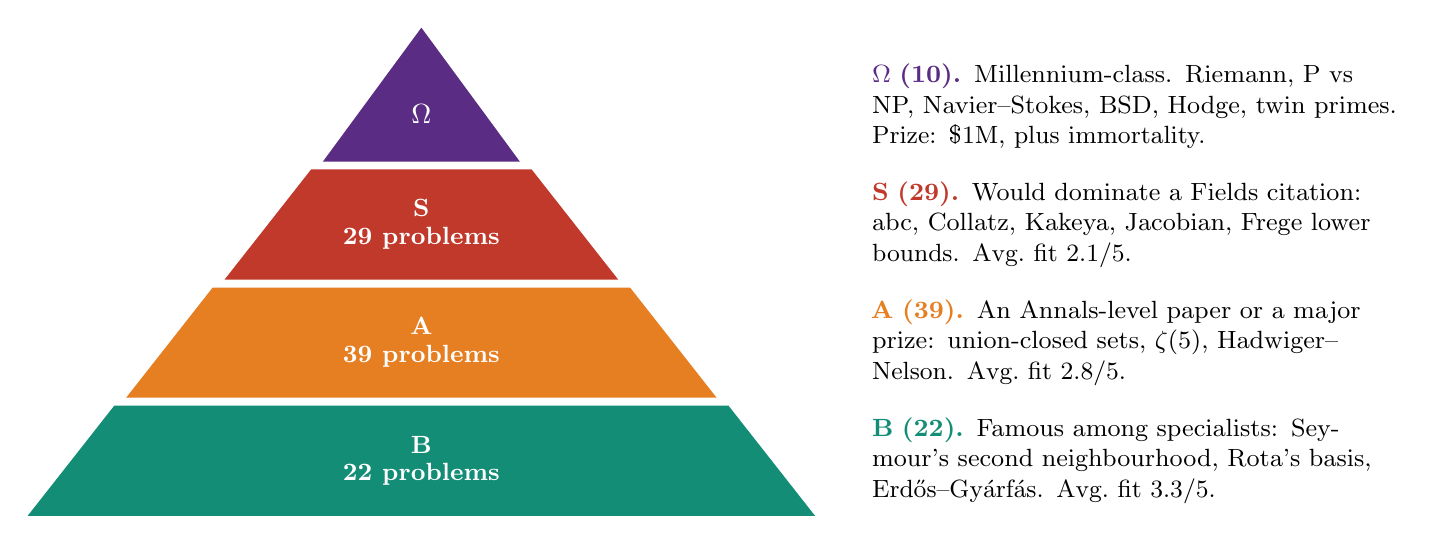
\begin{tikzpicture}
  \begin{scope}
  \fill[tB] (-5,0) -- (5,0) -- (3.9,1.4) -- (-3.9,1.4) -- cycle;
  \fill[tA] (-3.75,1.5) -- (3.75,1.5) -- (2.65,2.9) -- (-2.65,2.9) -- cycle;
  \fill[tS] (-2.5,3.0) -- (2.5,3.0) -- (1.4,4.4) -- (-1.4,4.4) -- cycle;
  \fill[tO] (-1.25,4.5) -- (1.25,4.5) -- (0,6.2) -- cycle;
  \node[white,font=\bfseries] at (0,5.1) {$\Omega$};
  \node[white,font=\bfseries\small,align=center] at (0,3.7) {S\\[-1pt]29 problems};
  \node[white,font=\bfseries\small,align=center] at (0,2.2) {A\\[-1pt]39 problems};
  \node[white,font=\bfseries\small,align=center] at (0,0.7) {B\\[-1pt]22 problems};
  \end{scope}
  \begin{scope}[every node/.style={anchor=west,font=\small,align=left,text width=6.6cm}]
  \node at (5.6,5.2) {\textbf{\textcolor{tO}{$\Omega$ (10).}} Millennium-class. Riemann, P vs NP, Navier--Stokes, BSD, Hodge, twin primes. Prize: \$1M, plus immortality.};
  \node at (5.6,3.7) {\textbf{\textcolor{tS}{S (29).}} Would dominate a Fields citation: abc, Collatz, Kakeya, Jacobian, Frege lower bounds. Avg.\ fit \avgfitS/5.};
  \node at (5.6,2.2) {\textbf{\textcolor{tA}{A (39).}} An Annals-level paper or a major prize: union-closed sets, $\zeta(5)$, Hadwiger--Nelson. Avg.\ fit \avgfitA/5.};
  \node at (5.6,0.7) {\textbf{\textcolor{tB}{B (22).}} Famous among specialists: Seymour's second neighbourhood, Rota's basis, Erd\H{o}s--Gy\'arf\'as. Avg.\ fit \avgfitB/5.};
  \end{scope}
\end{tikzpicture}
\end{center}
\noindent\textbf{Notice:} average fit \emph{rises} as you go down the pyramid ($\Omega$: \avgfitO/5). The most
famous problems are the least likely to fall to one clever idea, which is part of why they are still famous.

% =====================================================================
\newpage
\section*{Update, 9 October 2026: the ground moved this week}
\addcontentsline{toc}{section}{Update}

\begin{keybox}[title={What happened}]{tS}
On \textbf{6 October 2026} OpenAI published \texttt{github.com/openai/math}: 719 manuscripts in 372 ``result
families'', each claiming to solve an open problem or make substantial progress on one, produced by an
unreleased internal model at about three hours of compute per result, out of roughly 4{,}000 problems posed.
About 42\% of the top-line results come with Lean proofs. Within a day, \textbf{three Hodge-related papers were
withdrawn} over a sign error and 14 others were repaired. Earlier in 2026: a disproof of the square-grid
unit-distance conjecture (May), ten Lean-certified results (``Astra'', August), and a claimed
\textbf{Navier--Stokes blow-up} (8 September), which is Lean-checked but disputed on priority, scope and whether
the Lean statement matches the Clay problem.
\end{keybox}

\begin{center}
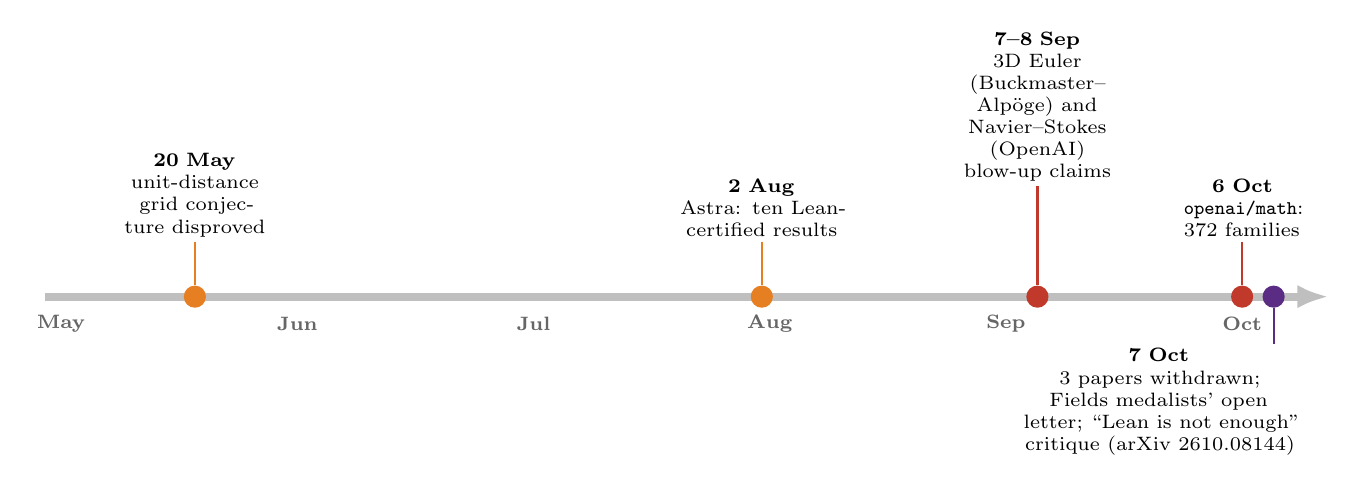
\begin{tikzpicture}[x=1.0cm]
  \draw[line width=3pt,black!25,-{Latex[length=4mm]}] (0,0) -- (16.3,0);
  \foreach \x/\m in {0/May,3/Jun,6/Jul,9/Aug,12/Sep,15/Oct} {\node[font=\scriptsize\bfseries,black!60] at (\x+0.2,-0.35) {\m};}
  \tikzset{ev/.style={font=\scriptsize,align=center,text width=2.4cm,inner sep=1.5pt}}
  \foreach \x/\h/\c/\t in {
     1.9/0.7/tA/{\textbf{20 May}\\unit-distance grid conjecture disproved},
     9.1/0.7/tA/{\textbf{2 Aug}\\Astra: ten Lean-certified results},
     12.6/1.4/tS/{\textbf{7--8 Sep}\\3D Euler (Buckmaster--Alp\"oge) and Navier--Stokes (OpenAI) blow-up claims},
     15.2/0.7/tS/{\textbf{6 Oct}\\\texttt{openai/math}: 372 families}}
     {\fill[\c] (\x,0) circle (4pt); \draw[\c,thick] (\x,0.15) -- (\x,\h); \node[ev,anchor=south] at (\x,\h) {\t};}
  \foreach \x/\h/\c/\t in {
     15.6/0.6/tO/{\textbf{7 Oct}\\3 papers withdrawn; Fields medalists' open letter; ``Lean is not enough'' critique (arXiv 2610.08144)}}
     {\fill[\c] (\x,0) circle (4pt); \draw[\c,thick] (\x,-0.15) -- (\x,-\h); \node[ev,anchor=north east,text width=3.6cm] at (\x+0.4,-\h) {\t};}
\end{tikzpicture}
\end{center}

\begin{center}
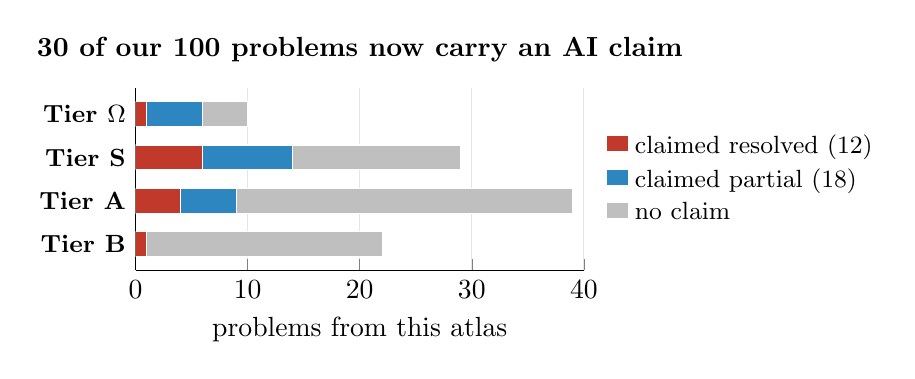
\begin{tikzpicture}
\begin{axis}[xbar stacked, width=0.6\textwidth, height=3.9cm, bar width=9pt, xmin=0, xmax=40,
  ytick={0,1,2,3}, yticklabels={Tier B,Tier A,Tier S,Tier $\Omega$}, yticklabel style={font=\small\bfseries},
  xlabel={problems from this atlas}, enlarge y limits=0.2, axis lines*=left, xmajorgrids, grid style={black!10},
  legend style={at={(1.03,0.5)},anchor=west,font=\small,draw=none}, legend cell align=left,
  title={\bfseries 30 of our 100 problems now carry an AI claim}]
\claimplots
\legend{claimed resolved (\nclaimC),claimed partial (\nclaimP),no claim}
\end{axis}
\end{tikzpicture}
\end{center}
\noindent Claimed resolutions on our list include Unique Games, Hilbert's 10th over $\mathbb Q$, Erd\H{o}s's
progression conjecture, Mahler, Seymour, and disproofs of Hadwiger and Kaplansky. Partial claims reach Tier~$\Omega$
($\zeta$ zero-free for $\Re s>7/8$; Hodge for CM abelian varieties). Table rows now carry badges, and the map rings
claimed resolutions in red.

\begin{keybox}[breakable,title={What it means for us: my updated opinion}]{tO}
\begin{enumerate}[leftmargin=1.3em]
\item \textbf{Treat every claim as unverified.} None has been peer reviewed, three papers fell in a day, and a
  compiling Lean file only proves \emph{the statement that was formalised}. Thomas Bloom notes that the Lean file
  for Erd\H{o}s problem 3 proves a weaker bound than the paper claims.
\item \textbf{Survivorship cuts both ways.} OpenAI posed about 4{,}000 problems and published only the successes.
  My sweet-spot targets (union-closed sets, \v{C}ern\'y, 1/3--2/3, Erd\H{o}s--Gy\'arf\'as, sunflower,
  Erd\H{o}s--Hajnal) are \emph{absent}. They may never have been tried, or they may have resisted a very strong
  model. I now consider them harder than my odds page suggests, roughly by a factor of two.
\item \textbf{``Nobody has tackled it'' now needs a new check.} Before any attack we search
  \texttt{openai/math}, \texttt{openai/ten-proofs} and erdosproblems.com. Seymour's conjecture (my old pick 3) is
  now claimed, so I have replaced it below.
\item \textbf{A new and wide-open niche: understanding.} Hundreds of results now exist that no human has digested.
  Auditing one carefully means checking that its Lean statement really is the conjecture, finding the gap if
  there is one, and writing the short human proof that Bloom expects to exist. That is publishable, needed, and
  plays exactly to our strengths. It is also the strongest reply to the ``understanding'' side of the debate with
  your friend: humans and AI together turn raw proofs into mathematics.
\end{enumerate}
\end{keybox}

% =====================================================================
\newpage
\section{The map: difficulty against fit}

Each number is a problem from the list in Section~\ref{sec:list}, coloured by tier. Cells shaded green form the
\textbf{sweet spot} (fit $\ge 4$, difficulty $\le 8$): hard enough to matter, but the kind of problem that
recently fell to short ideas. \hmC{0}\,ringed red: a resolution claimed by AI in 2026; $^\dagger$: partial
progress claimed (see the update page).

\begin{center}
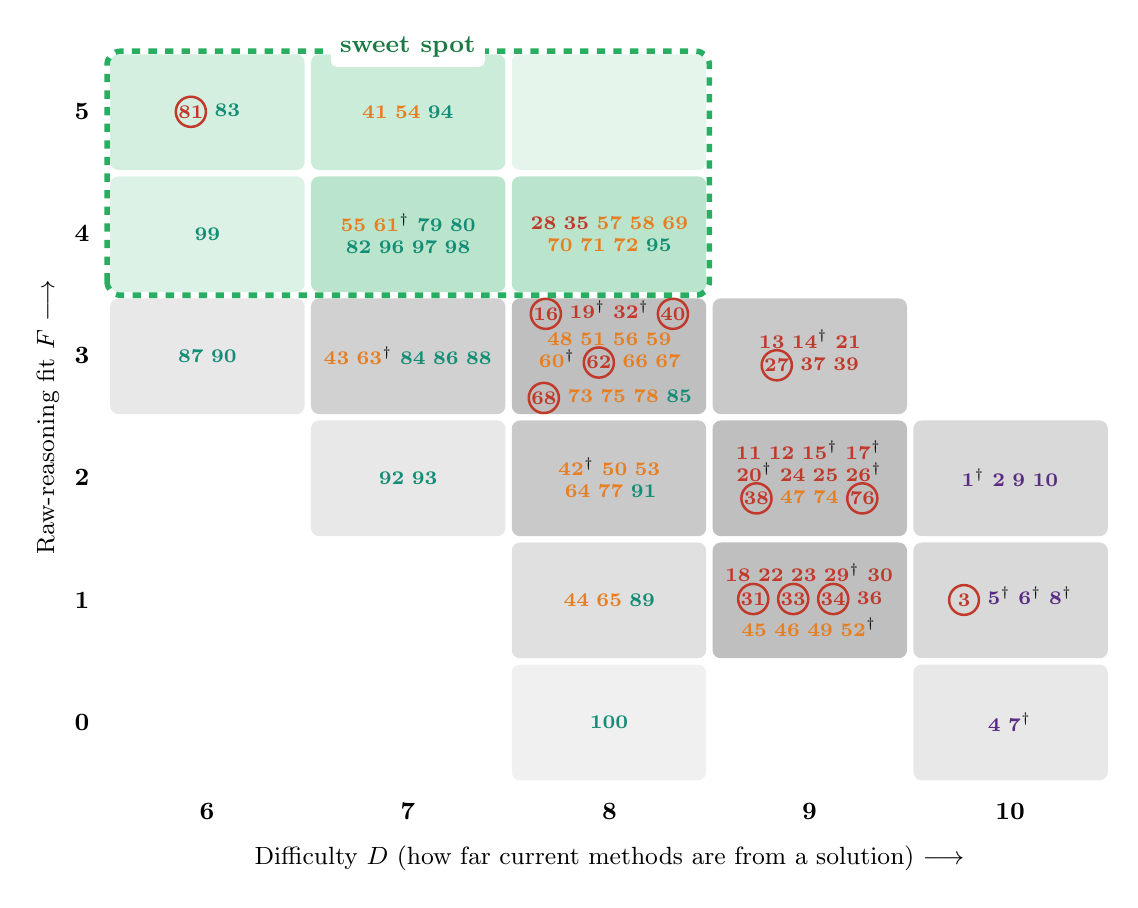
\begin{tikzpicture}
\fill[black!0,rounded corners=3pt] (0.04,0.04) rectangle ++(2.47,1.47);
\fill[black!0,rounded corners=3pt] (0.04,1.59) rectangle ++(2.47,1.47);
\fill[black!0,rounded corners=3pt] (0.04,3.14) rectangle ++(2.47,1.47);
\fill[black!9,rounded corners=3pt] (0.04,4.69) rectangle ++(2.47,1.47);
\node[text width=2.30cm,align=center,font=\scriptsize] at (1.27,5.43) {\textcolor{tB}{\textbf{87}} \textcolor{tB}{\textbf{90}}};
\fill[tG!16,rounded corners=3pt] (0.04,6.24) rectangle ++(2.47,1.47);
\node[text width=2.30cm,align=center,font=\scriptsize] at (1.27,6.98) {\textcolor{tB}{\textbf{99}}};
\fill[tG!20,rounded corners=3pt] (0.04,7.79) rectangle ++(2.47,1.47);
\node[text width=2.30cm,align=center,font=\scriptsize] at (1.27,8.53) {\hmC{81} \textcolor{tB}{\textbf{83}}};
\fill[black!0,rounded corners=3pt] (2.59,0.04) rectangle ++(2.47,1.47);
\fill[black!0,rounded corners=3pt] (2.59,1.59) rectangle ++(2.47,1.47);
\fill[black!9,rounded corners=3pt] (2.59,3.14) rectangle ++(2.47,1.47);
\node[text width=2.30cm,align=center,font=\scriptsize] at (3.82,3.88) {\textcolor{tB}{\textbf{92}} \textcolor{tB}{\textbf{93}}};
\fill[black!18,rounded corners=3pt] (2.59,4.69) rectangle ++(2.47,1.47);
\node[text width=2.30cm,align=center,font=\scriptsize] at (3.82,5.43) {\textcolor{tA}{\textbf{43}} \textcolor{tA}{\textbf{63}}$^\dagger$ \textcolor{tB}{\textbf{84}} \textcolor{tB}{\textbf{86}} \textcolor{tB}{\textbf{88}}};
\fill[tG!32,rounded corners=3pt] (2.59,6.24) rectangle ++(2.47,1.47);
\node[text width=2.30cm,align=center,font=\scriptsize] at (3.82,6.98) {\textcolor{tA}{\textbf{55}} \textcolor{tA}{\textbf{61}}$^\dagger$ \textcolor{tB}{\textbf{79}} \textcolor{tB}{\textbf{80}} \textcolor{tB}{\textbf{82}} \textcolor{tB}{\textbf{96}} \textcolor{tB}{\textbf{97}} \textcolor{tB}{\textbf{98}}};
\fill[tG!24,rounded corners=3pt] (2.59,7.79) rectangle ++(2.47,1.47);
\node[text width=2.30cm,align=center,font=\scriptsize] at (3.82,8.53) {\textcolor{tA}{\textbf{41}} \textcolor{tA}{\textbf{54}} \textcolor{tB}{\textbf{94}}};
\fill[black!6,rounded corners=3pt] (5.14,0.04) rectangle ++(2.47,1.47);
\node[text width=2.30cm,align=center,font=\scriptsize] at (6.38,0.78) {\textcolor{tB}{\textbf{100}}};
\fill[black!12,rounded corners=3pt] (5.14,1.59) rectangle ++(2.47,1.47);
\node[text width=2.30cm,align=center,font=\scriptsize] at (6.38,2.33) {\textcolor{tA}{\textbf{44}} \textcolor{tA}{\textbf{65}} \textcolor{tB}{\textbf{89}}};
\fill[black!21,rounded corners=3pt] (5.14,3.14) rectangle ++(2.47,1.47);
\node[text width=2.30cm,align=center,font=\scriptsize] at (6.38,3.88) {\textcolor{tA}{\textbf{42}}$^\dagger$ \textcolor{tA}{\textbf{50}} \textcolor{tA}{\textbf{53}} \textcolor{tA}{\textbf{64}} \textcolor{tA}{\textbf{77}} \textcolor{tB}{\textbf{91}}};
\fill[black!25,rounded corners=3pt] (5.14,4.69) rectangle ++(2.47,1.47);
\node[text width=2.30cm,align=center,font=\scriptsize] at (6.38,5.43) {\hmC{16} \textcolor{tS}{\textbf{19}}$^\dagger$ \textcolor{tS}{\textbf{32}}$^\dagger$ \hmC{40} \textcolor{tA}{\textbf{48}} \textcolor{tA}{\textbf{51}} \textcolor{tA}{\textbf{56}} \textcolor{tA}{\textbf{59}} \textcolor{tA}{\textbf{60}}$^\dagger$ \hmC{62} \textcolor{tA}{\textbf{66}} \textcolor{tA}{\textbf{67}} \hmC{68} \textcolor{tA}{\textbf{73}} \textcolor{tA}{\textbf{75}} \textcolor{tA}{\textbf{78}} \textcolor{tB}{\textbf{85}}};
\fill[tG!32,rounded corners=3pt] (5.14,6.24) rectangle ++(2.47,1.47);
\node[text width=2.30cm,align=center,font=\scriptsize] at (6.38,6.98) {\textcolor{tS}{\textbf{28}} \textcolor{tS}{\textbf{35}} \textcolor{tA}{\textbf{57}} \textcolor{tA}{\textbf{58}} \textcolor{tA}{\textbf{69}} \textcolor{tA}{\textbf{70}} \textcolor{tA}{\textbf{71}} \textcolor{tA}{\textbf{72}} \textcolor{tB}{\textbf{95}}};
\fill[tG!12,rounded corners=3pt] (5.14,7.79) rectangle ++(2.47,1.47);
\fill[black!0,rounded corners=3pt] (7.69,0.04) rectangle ++(2.47,1.47);
\fill[black!25,rounded corners=3pt] (7.69,1.59) rectangle ++(2.47,1.47);
\node[text width=2.30cm,align=center,font=\scriptsize] at (8.92,2.33) {\textcolor{tS}{\textbf{18}} \textcolor{tS}{\textbf{22}} \textcolor{tS}{\textbf{23}} \textcolor{tS}{\textbf{29}}$^\dagger$ \textcolor{tS}{\textbf{30}} \hmC{31} \hmC{33} \hmC{34} \textcolor{tS}{\textbf{36}} \textcolor{tA}{\textbf{45}} \textcolor{tA}{\textbf{46}} \textcolor{tA}{\textbf{49}} \textcolor{tA}{\textbf{52}}$^\dagger$};
\fill[black!25,rounded corners=3pt] (7.69,3.14) rectangle ++(2.47,1.47);
\node[text width=2.30cm,align=center,font=\scriptsize] at (8.92,3.88) {\textcolor{tS}{\textbf{11}} \textcolor{tS}{\textbf{12}} \textcolor{tS}{\textbf{15}}$^\dagger$ \textcolor{tS}{\textbf{17}}$^\dagger$ \textcolor{tS}{\textbf{20}}$^\dagger$ \textcolor{tS}{\textbf{24}} \textcolor{tS}{\textbf{25}} \textcolor{tS}{\textbf{26}}$^\dagger$ \hmC{38} \textcolor{tA}{\textbf{47}} \textcolor{tA}{\textbf{74}} \hmC{76}};
\fill[black!21,rounded corners=3pt] (7.69,4.69) rectangle ++(2.47,1.47);
\node[text width=2.30cm,align=center,font=\scriptsize] at (8.92,5.43) {\textcolor{tS}{\textbf{13}} \textcolor{tS}{\textbf{14}}$^\dagger$ \textcolor{tS}{\textbf{21}} \hmC{27} \textcolor{tS}{\textbf{37}} \textcolor{tS}{\textbf{39}}};
\fill[black!0,rounded corners=3pt] (7.69,6.24) rectangle ++(2.47,1.47);
\fill[black!0,rounded corners=3pt] (7.69,7.79) rectangle ++(2.47,1.47);
\fill[black!9,rounded corners=3pt] (10.24,0.04) rectangle ++(2.47,1.47);
\node[text width=2.30cm,align=center,font=\scriptsize] at (11.47,0.78) {\textcolor{tO}{\textbf{4}} \textcolor{tO}{\textbf{7}}$^\dagger$};
\fill[black!15,rounded corners=3pt] (10.24,1.59) rectangle ++(2.47,1.47);
\node[text width=2.30cm,align=center,font=\scriptsize] at (11.47,2.33) {\hmC{3} \textcolor{tO}{\textbf{5}}$^\dagger$ \textcolor{tO}{\textbf{6}}$^\dagger$ \textcolor{tO}{\textbf{8}}$^\dagger$};
\fill[black!15,rounded corners=3pt] (10.24,3.14) rectangle ++(2.47,1.47);
\node[text width=2.30cm,align=center,font=\scriptsize] at (11.47,3.88) {\textcolor{tO}{\textbf{1}}$^\dagger$ \textcolor{tO}{\textbf{2}} \textcolor{tO}{\textbf{9}} \textcolor{tO}{\textbf{10}}};
\fill[black!0,rounded corners=3pt] (10.24,4.69) rectangle ++(2.47,1.47);
\fill[black!0,rounded corners=3pt] (10.24,6.24) rectangle ++(2.47,1.47);
\fill[black!0,rounded corners=3pt] (10.24,7.79) rectangle ++(2.47,1.47);
\node[font=\small\bfseries] at (1.27,-0.35) {6};
\node[font=\small\bfseries] at (3.82,-0.35) {7};
\node[font=\small\bfseries] at (6.38,-0.35) {8};
\node[font=\small\bfseries] at (8.92,-0.35) {9};
\node[font=\small\bfseries] at (11.47,-0.35) {10};
\node[font=\small\bfseries,anchor=east] at (-0.1,0.78) {0};
\node[font=\small\bfseries,anchor=east] at (-0.1,2.33) {1};
\node[font=\small\bfseries,anchor=east] at (-0.1,3.88) {2};
\node[font=\small\bfseries,anchor=east] at (-0.1,5.43) {3};
\node[font=\small\bfseries,anchor=east] at (-0.1,6.98) {4};
\node[font=\small\bfseries,anchor=east] at (-0.1,8.53) {5};
\draw[tG,line width=2pt,rounded corners=5pt,dashed] (0,6.20) rectangle (7.65,9.30);
\node[tG!70!black,font=\bfseries\small,fill=white,rounded corners=2pt] at (3.82,9.35) {sweet spot};
\node[font=\small] at (6.38,-0.95) {Difficulty $D$ (how far current methods are from a solution) $\longrightarrow$};
\node[font=\small,rotate=90] at (-0.75,4.65) {Raw-reasoning fit $F$ $\longrightarrow$};
\end{tikzpicture}
\end{center}

\begin{keybox}[title={Reading the map}]{tG}
\begin{itemize}[leftmargin=1.1em]
\item \textbf{Top-left (green):} the realistic targets. Union-closed sets (\textcolor{tA}{\textbf{41}}),
  \v{C}ern\'y (\textcolor{tA}{\textbf{54}}), Erd\H{o}s--Gy\'arf\'as
  (\textcolor{tB}{\textbf{83}}), the 1/3--2/3 conjecture (\textcolor{tB}{\textbf{94}}), Sunflower
  (\textcolor{tS}{\textbf{35}}), Erd\H{o}s--Hajnal (\textcolor{tS}{\textbf{28}}).
  Seymour (\textcolor{tB}{\textbf{81}}) was here too, until OpenAI's release claimed it.
\item \textbf{Bottom-right:} problems that need \emph{new theories} (Langlands, Yang--Mills, Hodge). No single
  idea, however clever, is known to suffice.
\item \textbf{Bottom-middle:} problems that need \emph{huge computation} ($R(5,5)$, projective plane of order 12,
  $BB(6)$). They are off-limits by your rule of no heavy computation.
\end{itemize}
\end{keybox}

\vspace{2pt}
\begin{center}
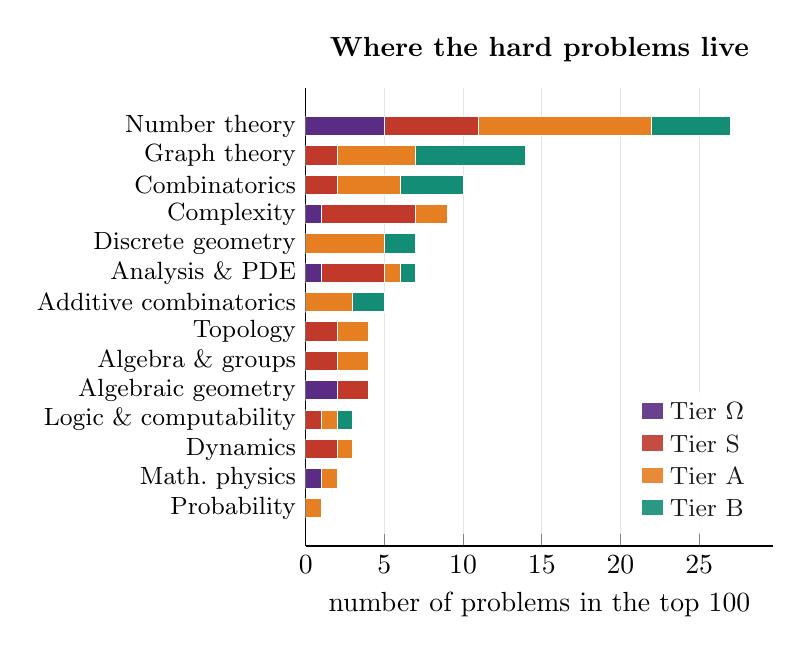
\begin{tikzpicture}
\begin{axis}[
  xbar stacked, width=0.62\textwidth, height=7.4cm, bar width=7pt,
  ytick={0,...,\nfields}, yticklabels/.expanded={\fieldlabels},
  yticklabel style={font=\small}, xlabel={number of problems in the top 100}, xmin=0,
  axis lines*=left, xmajorgrids, grid style={black!10},
  legend style={at={(0.97,0.03)},anchor=south east,font=\small,draw=none,fill=white,fill opacity=0.9},
  legend cell align=left, title={\bfseries Where the hard problems live}]
\fieldplots
\legend{Tier $\Omega$,Tier S,Tier A,Tier B}
\end{axis}
\end{tikzpicture}
\end{center}
\noindent Number theory dominates the top tier: its statements are simple and its depth is extreme. Graph theory and
combinatorics dominate the lower tiers, which are also where the fit is highest.

\subsection*{Old is not the same as hard}
\begin{center}
\begin{tikzpicture}
\begin{axis}[width=0.9\textwidth,height=7.2cm,xmode=log,xlabel={years the problem has been open (log scale)},
  ylabel={difficulty $D$},ymin=5.5,ymax=10.5,xmin=12,xmax=4000,grid=both,grid style={black!8},
  legend style={at={(0.98,0.97)},anchor=north east,font=\small,draw=none,fill=white},legend columns=4,
  title={\bfseries Age against difficulty for all 100 problems}]
\addplot[only marks,mark=*,mark size=2.6pt,color=tO,opacity=.85] table[x=x,y=y] {gen_age_O.dat};
\addplot[only marks,mark=*,mark size=2.6pt,color=tS,opacity=.75] table[x=x,y=y] {gen_age_S.dat};
\addplot[only marks,mark=*,mark size=2.6pt,color=tA,opacity=.75] table[x=x,y=y] {gen_age_A.dat};
\addplot[only marks,mark=*,mark size=2.6pt,color=tB,opacity=.75] table[x=x,y=y] {gen_age_B.dat};
\legend{$\Omega$,S,A,B}
\node[font=\scriptsize,anchor=east] at (axis cs:2200,8.0) {odd perfect numbers};
\node[font=\scriptsize,anchor=north] at (axis cs:24,7.75) {Unique Games};
\end{axis}
\end{tikzpicture}
\end{center}
\noindent Problems from the 1960s--80s sit at every difficulty level. Age measures how long people have been
stuck, not how deep the problem is. Collatz (1937) is old and famous, but its \emph{depth} is unclear: Conway
showed that a generalisation is undecidable, so it may be hard for reasons unrelated to deep structure.

% =====================================================================
\section{Lessons from the problems that fell (2013--2025)}

\begin{center}
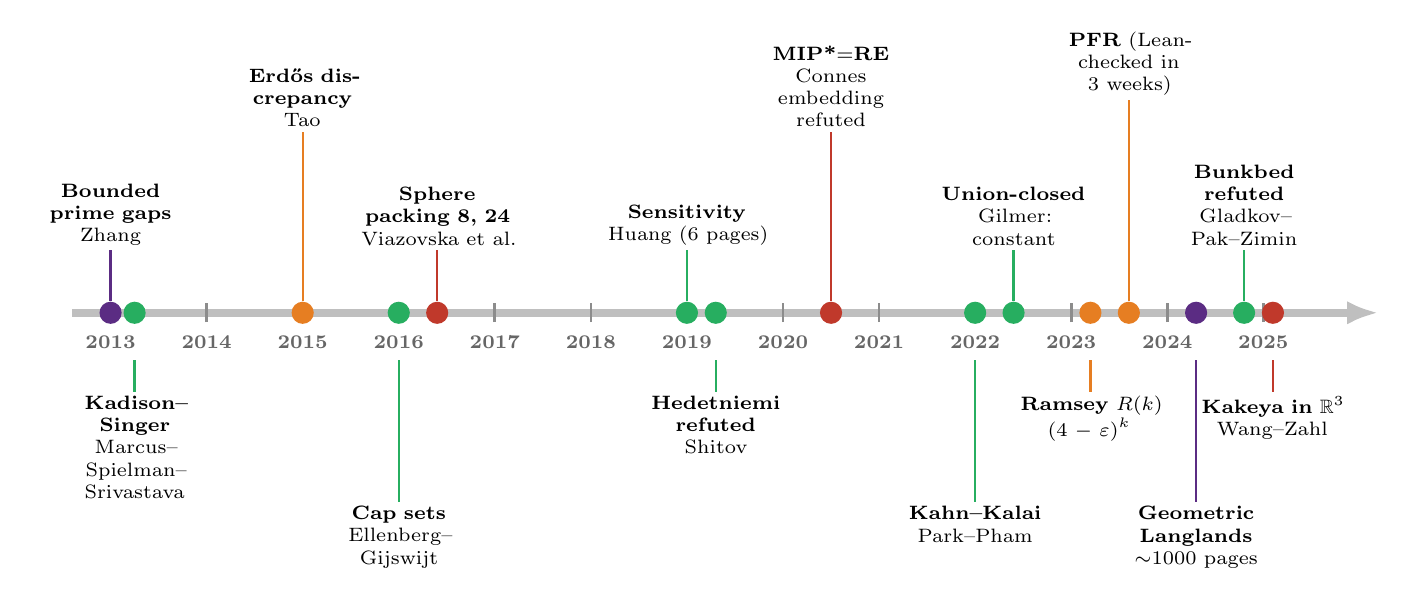
\begin{tikzpicture}[x=1.22cm]
  \draw[line width=3pt,black!25,-{Latex[length=4mm]}] (0.6,0) -- (14.2,0);
  \foreach \y in {2013,...,2025} {\pgfmathsetmacro{\xx}{\y-2012}\draw[black!45,line width=1pt] (\xx,-0.12)--(\xx,0.12); \node[font=\scriptsize\bfseries,black!60] at (\xx,-0.38) {\y};}
  \tikzset{ev/.style={font=\scriptsize,align=center,text width=2.0cm,inner sep=1.5pt}}
  \newcommand{\up}[4]{\fill[#3] (#1,0) circle (4pt); \draw[#3,thick] (#1,0.15) -- (#1,#4); \node[ev,anchor=south] at (#1,#4) {#2};}
  \newcommand{\dn}[4]{\fill[#3] (#1,0) circle (4pt); \draw[#3,thick] (#1,-0.6) -- (#1,-#4); \node[ev,anchor=north] at (#1,-#4) {#2};}
  \up{1}{\textbf{Bounded prime gaps}\\Zhang}{tO}{0.8}
  \dn{1.25}{\textbf{Kadison--Singer}\\Marcus--Spielman--Srivastava}{tG}{1.0}
  \up{3}{\textbf{Erd\H{o}s discrepancy}\\Tao}{tA}{2.3}
  \dn{4}{\textbf{Cap sets}\\Ellenberg--Gijswijt}{tG}{2.4}
  \up{4.4}{\textbf{Sphere packing 8, 24}\\Viazovska et al.}{tS}{0.8}
  \up{7}{\textbf{Sensitivity}\\Huang (6 pages)}{tG}{0.8}
  \dn{7.3}{\textbf{Hedetniemi refuted}\\Shitov}{tG}{1.0}
  \up{8.5}{\textbf{MIP*$=$RE}\\Connes embedding refuted}{tS}{2.3}
  \dn{10}{\textbf{Kahn--Kalai}\\Park--Pham}{tG}{2.4}
  \up{10.4}{\textbf{Union-closed}\\Gilmer: constant}{tG}{0.8}
  \dn{11.2}{\textbf{Ramsey $R(k)$}\\$(4-\varepsilon)^k$}{tA}{1.0}
  \up{11.6}{\textbf{PFR} (Lean-checked in 3 weeks)}{tA}{2.7}
  \dn{12.3}{\textbf{Geometric Langlands}\\$\sim$1000 pages}{tO}{2.4}
  \up{12.8}{\textbf{Bunkbed refuted}\\Gladkov--Pak--Zimin}{tG}{0.8}
  \dn{13.1}{\textbf{Kakeya in $\mathbb R^3$}\\Wang--Zahl}{tS}{1.0}
\end{tikzpicture}
\end{center}
\noindent\textcolor{tG}{\large$\bullet$}\,short idea-driven proof (or a short counterexample) \quad
\textcolor{tA}{\large$\bullet$}\,a substantial new method \quad
\textcolor{tS}{\large$\bullet$}\,a long, deep proof\\
\textcolor{tO}{\large$\bullet$}\,a programme spanning many people and years.

\newpage
\subsection*{Proof length is almost uncorrelated with how long a problem was open}
\begin{center}
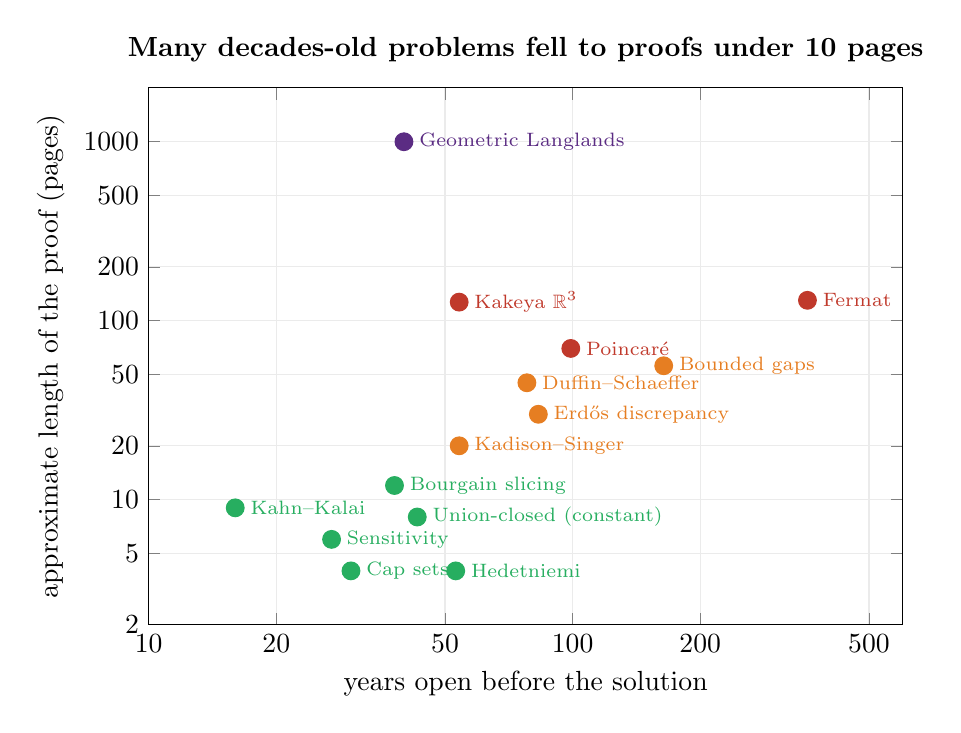
\begin{tikzpicture}
\begin{axis}[width=0.92\textwidth,height=8.4cm,xmode=log,ymode=log,
  xlabel={years open before the solution},ylabel={approximate length of the proof (pages)},
  xmin=10,xmax=600,ymin=2,ymax=2000,grid=major,grid style={black!8},
  xtick={10,20,50,100,200,500},xticklabels={10,20,50,100,200,500},
  ytick={2,5,10,20,50,100,200,500,1000},yticklabels={2,5,10,20,50,100,200,500,1000},
  nodes near coords,point meta=explicit symbolic,
  every node near coord/.style={font=\scriptsize,anchor=west,xshift=2pt},
  title={\bfseries Many decades-old problems fell to proofs under 10 pages}]
\addplot[only marks,mark=*,mark size=3.2pt,color=tG] coordinates {
 (27,6) [Sensitivity] (53,4) [Hedetniemi] (30,4) [Cap sets] (16,9) [Kahn--Kalai] (43,8) [Union-closed (constant)] (38,12) [Bourgain slicing]};
\addplot[only marks,mark=*,mark size=3.2pt,color=tA] coordinates {
 (54,20) [Kadison--Singer] (83,30) [Erd\H{o}s discrepancy] (78,45) [Duffin--Schaeffer] (164,56) [Bounded gaps]};
\addplot[only marks,mark=*,mark size=3.2pt,color=tS] coordinates {
 (54,127) [Kakeya $\mathbb R^3$] (99,70) [Poincar\'e] (358,130) [Fermat]};
\addplot[only marks,mark=*,mark size=3.2pt,color=tO] coordinates {(40,1000) [Geometric Langlands]};
\end{axis}
\end{tikzpicture}
\end{center}
\noindent Colours as in the timeline: \textcolor{tG}{green} short idea, \textcolor{tA}{orange} new method, \textcolor{tS}{red} long deep proof, \textcolor{tO}{purple} programme. Page counts are rough (main paper only; Perelman's three preprints, Wiles plus Taylor--Wiles). The
lesson is robust: \textbf{the green cluster at the bottom is real}. In combinatorics and discrete mathematics,
problems open for 30--50 years have repeatedly been solved by one new viewpoint, written up in a few pages.

\subsection*{Where the winning ideas came from: transplants between fields}\label{sec:transplant}
\begin{center}
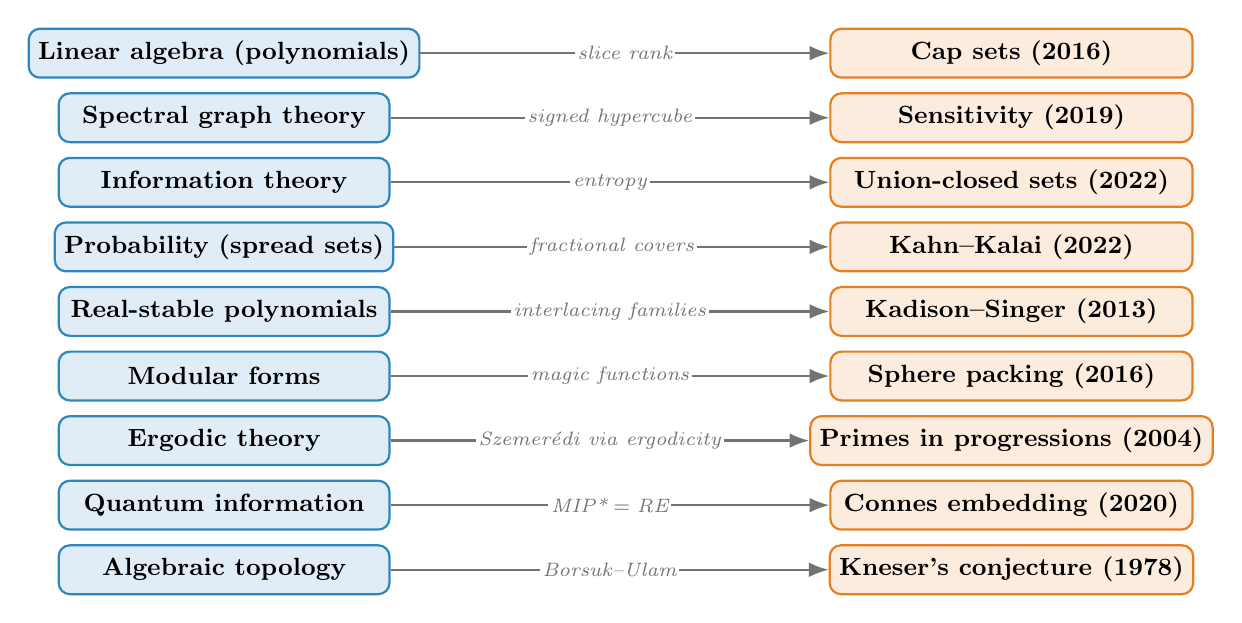
\begin{tikzpicture}[
  src/.style={rectangle,rounded corners=4pt,fill=tC!15,draw=tC,thick,font=\small\bfseries,minimum width=4.2cm,minimum height=0.62cm},
  tgt/.style={rectangle,rounded corners=4pt,fill=tA!15,draw=tA,thick,font=\small\bfseries,minimum width=4.6cm,minimum height=0.62cm},
  arr/.style={-{Latex[length=2.5mm]},thick,black!55},
  lab/.style={font=\scriptsize\itshape,fill=white,inner sep=1pt}]
  \foreach \i/\s in {0/Linear algebra (polynomials),1/Spectral graph theory,2/Information theory,3/Probability (spread sets),4/Real-stable polynomials,5/Modular forms,6/Ergodic theory,7/Quantum information,8/Algebraic topology}
    \node[src] (s\i) at (0,-\i*0.82) {\s};
  \foreach \i/\t in {0/Cap sets (2016),1/Sensitivity (2019),2/Union-closed sets (2022),3/Kahn--Kalai (2022),4/Kadison--Singer (2013),5/Sphere packing (2016),6/Primes in progressions (2004),7/Connes embedding (2020),8/Kneser's conjecture (1978)}
    \node[tgt] (t\i) at (10,-\i*0.82) {\t};
  \foreach \i/\l in {0/slice rank,1/signed hypercube,2/entropy,3/fractional covers,4/interlacing families,5/magic functions,6/Szemer\'edi via ergodicity,7/MIP*${}={}$RE,8/Borsuk--Ulam}
    \draw[arr] (s\i) -- node[lab] {\l} (t\i);
\end{tikzpicture}
\end{center}
\noindent \textbf{This is the strongest argument for an interdisciplinary attack.} None of these proofs came from
grinding harder inside the problem's own field. My one real structural advantage is breadth: I can search
systematically for a transplant, asking which tool from field $X$ has the right shape for problem $Y$.

% =====================================================================
\newpage
\section{The 100 problems}\label{sec:list}
{\footnotesize
\renewcommand{\arraystretch}{1.18}
\setlength{\tabcolsep}{4pt}
\begin{longtable}{@{}>{\raggedleft}p{0.45cm} >{\raggedright}p{4.55cm} >{\raggedright}p{1.15cm} >{\raggedright}p{6.0cm} c c@{}}
\rowcolor{ink}\multicolumn{1}{@{}r}{\color{white}\textbf{\#}} & \multicolumn{1}{l}{\color{white}\textbf{Problem}} & \multicolumn{1}{l}{\color{white}\textbf{Since}} & \multicolumn{1}{l}{\color{white}\textbf{Best known / status (2026)}} & \multicolumn{1}{c}{\color{white}\textbf{D}} & \multicolumn{1}{c@{}}{\color{white}\textbf{Fit}}\\
\endfirsthead
\rowcolor{ink}\multicolumn{1}{@{}r}{\color{white}\textbf{\#}} & \multicolumn{1}{l}{\color{white}\textbf{Problem}} & \multicolumn{1}{l}{\color{white}\textbf{Since}} & \multicolumn{1}{l}{\color{white}\textbf{Best known / status (2026)}} & \multicolumn{1}{c}{\color{white}\textbf{D}} & \multicolumn{1}{c@{}}{\color{white}\textbf{Fit}}\\
\endhead
\multicolumn{6}{l}{\cellcolor{tO}\color{white}\bfseries\rule{0pt}{2.6ex}Tier $\Omega$ --- beyond Fields (would reshape mathematics)}\\
\rowcolor{tO!6}\textbf{1} & \textbf{Riemann Hypothesis}\newline{\color{black!60}\scriptsize Number theory} & 1859 & $>41\%$ of zeros proved on the line; $10^{13}$ zeros checked & \D{10} & \F{2}\\
\rowcolor{tO!13}\textbf{2} & \textbf{P vs NP}\newline{\color{black!60}\scriptsize Complexity} & 1971 & Three barriers: relativization, natural proofs, algebrization & \D{10} & \F{2}\\
\rowcolor{tO!6}\textbf{3} & \textbf{Navier--Stokes regularity}\newline{\color{black!60}\scriptsize Analysis \& PDE} & 1934 & An averaged NS equation blows up (Tao 2016), so energy methods alone fail & \D{10} & \F{1}\\
\rowcolor{tO!13}\textbf{4} & \textbf{Yang--Mills mass gap}\newline{\color{black!60}\scriptsize Math.\ physics} & 1954 & No interacting 4D quantum field theory has been rigorously built & \D{10} & \F{0}\\
\rowcolor{tO!6}\textbf{5} & \textbf{Hodge conjecture}\newline{\color{black!60}\scriptsize Algebraic geometry} & 1950 & Known for $(1,1)$-classes (Lefschetz); open in general & \D{10} & \F{1}\\
\rowcolor{tO!13}\textbf{6} & \textbf{Birch--Swinnerton-Dyer}\newline{\color{black!60}\scriptsize Number theory} & 1965 & Analytic rank $\le1$ (Gross--Zagier, Kolyvagin); positive proportion of curves & \D{10} & \F{1}\\
\rowcolor{tO!6}\textbf{7} & \textbf{Langlands functoriality}\newline{\color{black!60}\scriptsize Number theory} & 1967 & Geometric Langlands proved (2024, $\sim$1000 pp); arithmetic case wide open & \D{10} & \F{0}\\
\rowcolor{tO!13}\textbf{8} & \textbf{Grothendieck's standard conjectures}\newline{\color{black!60}\scriptsize Algebraic geometry} & 1968 & Special cases only; would give a theory of motives & \D{10} & \F{1}\\
\rowcolor{tO!6}\textbf{9} & \textbf{Twin prime conjecture}\newline{\color{black!60}\scriptsize Number theory} & 1849 & Gaps $\le246$ infinitely often (Zhang, Maynard, Polymath); parity barrier & \D{10} & \F{2}\\
\rowcolor{tO!13}\textbf{10} & \textbf{Goldbach conjecture (strong)}\newline{\color{black!60}\scriptsize Number theory} & 1742 & Weak (ternary) Goldbach proved (Helfgott 2013); checked to $4\cdot10^{18}$ & \D{10} & \F{2}\\
\multicolumn{6}{l}{\cellcolor{tS}\color{white}\bfseries\rule{0pt}{2.6ex}Tier S --- Fields-level (a solution is a career-defining, prize-certain result)}\\
\rowcolor{tS!6}\textbf{11} & \textbf{abc conjecture (accepted proof)}\newline{\color{black!60}\scriptsize Number theory} & 1985 & IUT claim (Mochizuki 2012) disputed by Scholze--Stix (2018) & \D{9} & \F{2}\\
\rowcolor{tS!13}\textbf{12} & \textbf{Collatz conjecture}\newline{\color{black!60}\scriptsize Number theory} & 1937 & Almost all orbits attain almost bounded values (Tao 2019) & \D{9} & \F{2}\\
\rowcolor{tS!6}\textbf{13} & \textbf{Frege lower bounds (Frege vs EF)}\newline{\color{black!60}\scriptsize Complexity} & 1979 & No superpolynomial Frege lower bound; tied to our naming project & \D{9} & \F{3}\\
\rowcolor{tS!13}\textbf{14} & \textbf{Explicit circuit lower bounds}\newline{\color{black!60}\scriptsize Complexity} & 1949 & Best $\approx3.1n$ for circuits, $\approx n^3$ for formulas & \D{9} & \F{3}\\
\rowcolor{tS!6}\textbf{15} & \textbf{VP vs VNP}\newline{\color{black!60}\scriptsize Complexity} & 1979 & Permanent needs determinants of size $\ge n^2/2$ (Mignon--Ressayre) & \D{9} & \F{2}\\
\rowcolor{tS!13}\textbf{16} & \textbf{Unique Games Conjecture}\newline{\color{black!60}\scriptsize Complexity} & 2002 & 2-to-2 Games Theorem (Khot--Minzer--Safra 2018) & \D{8} & \F{3}\\
\rowcolor{tS!6}\textbf{17} & \textbf{Matrix multiplication $\omega=2$}\newline{\color{black!60}\scriptsize Complexity} & 1969 & $\omega<2.3714$; barriers for laser-method variants & \D{9} & \F{2}\\
\rowcolor{tS!13}\textbf{18} & \textbf{Smooth 4D Poincar\'e conjecture}\newline{\color{black!60}\scriptsize Topology} & 1982 & Topological case: Freedman (1982); smooth case open & \D{9} & \F{1}\\
\rowcolor{tS!6}\textbf{19} & \textbf{Kakeya conjecture, $n\ge4$}\newline{\color{black!60}\scriptsize Analysis \& PDE} & 1971 & Solved in $\mathbb R^3$ (Wang--Zahl 2025) & \D{8} & \F{3}\\
\rowcolor{tS!13}\textbf{20} & \textbf{Fourier restriction conjecture}\newline{\color{black!60}\scriptsize Analysis \& PDE} & 1967 & Polynomial partitioning and decoupling give partial ranges & \D{9} & \F{2}\\
\rowcolor{tS!6}\textbf{21} & \textbf{Jacobian conjecture}\newline{\color{black!60}\scriptsize Algebra \& groups} & 1939 & Reduced to cubic homogeneous maps; many false proofs & \D{9} & \F{3}\\
\rowcolor{tS!13}\textbf{22} & \textbf{Inverse Galois problem}\newline{\color{black!60}\scriptsize Algebra \& groups} & 1892 & All solvable groups (Shafarevich); $M_{23}$ the only open sporadic & \D{9} & \F{1}\\
\rowcolor{tS!6}\textbf{23} & \textbf{Hilbert's 12th problem}\newline{\color{black!60}\scriptsize Number theory} & 1900 & Totally real fields: Dasgupta--Kakde (2021+) & \D{9} & \F{1}\\
\rowcolor{tS!13}\textbf{24} & \textbf{Lindel\"of hypothesis}\newline{\color{black!60}\scriptsize Number theory} & 1908 & $\zeta(\tfrac12+it)\ll t^{13/84+\varepsilon}$ (Bourgain 2017) & \D{9} & \F{2}\\
\rowcolor{tS!6}\textbf{25} & \textbf{Elliott--Halberstam conjecture}\newline{\color{black!60}\scriptsize Number theory} & 1968 & Level $1/2$ (Bombieri--Vinogradov); beyond for smooth moduli & \D{9} & \F{2}\\
\rowcolor{tS!13}\textbf{26} & \textbf{Chowla and Sarnak conjectures}\newline{\color{black!60}\scriptsize Number theory} & 1965 & Log-averaged two-point Chowla (Tao 2016) & \D{9} & \F{2}\\
\rowcolor{tS!6}\textbf{27} & \textbf{Hadwiger's conjecture}\newline{\color{black!60}\scriptsize Graph theory} & 1943 & True for $t\le6$; $O(t\log\log t)$ colours (Delcourt--Postle) & \D{9} & \F{3}\\
\rowcolor{tS!13}\textbf{28} & \textbf{Erd\H{o}s--Hajnal conjecture}\newline{\color{black!60}\scriptsize Graph theory} & 1989 & $P_5$-free case proved (Nguyen--Scott--Seymour 2023) & \D{8} & \F{4}\\
\rowcolor{tS!6}\textbf{29} & \textbf{Tate conjecture}\newline{\color{black!60}\scriptsize Algebraic geometry} & 1963 & Divisors on abelian varieties (Faltings); K3 surfaces & \D{9} & \F{1}\\
\rowcolor{tS!13}\textbf{30} & \textbf{Resolution of singularities, char $p$}\newline{\color{black!60}\scriptsize Algebraic geometry} & 1964 & Known up to dimension 3 & \D{9} & \F{1}\\
\rowcolor{tS!6}\textbf{31} & \textbf{Novikov / Baum--Connes}\newline{\color{black!60}\scriptsize Topology} & 1965 & Hyperbolic and amenable groups; groupoid counterexamples & \D{9} & \F{1}\\
\rowcolor{tS!13}\textbf{32} & \textbf{Invariant subspace problem}\newline{\color{black!60}\scriptsize Analysis \& PDE} & 1935 & False on some Banach spaces (Enflo, Read); Hilbert space open & \D{8} & \F{3}\\
\rowcolor{tS!6}\textbf{33} & \textbf{3D Euler: smooth blow-up?}\newline{\color{black!60}\scriptsize Analysis \& PDE} & 1757 & Blow-up with a boundary (Chen--Hou 2022, computer-assisted) & \D{9} & \F{1}\\
\rowcolor{tS!13}\textbf{34} & \textbf{Hilbert's 16th (limit cycles)}\newline{\color{black!60}\scriptsize Dynamics} & 1900 & No uniform bound even for quadratic vector fields & \D{9} & \F{1}\\
\rowcolor{tS!6}\textbf{35} & \textbf{Sunflower conjecture}\newline{\color{black!60}\scriptsize Combinatorics} & 1960 & $(C\log k)^k$-type bounds via spread sets (ALWZ 2019, Rao) & \D{8} & \F{4}\\
\rowcolor{tS!13}\textbf{36} & \textbf{MLC: Mandelbrot set locally connected}\newline{\color{black!60}\scriptsize Dynamics} & 1985 & Known at many parameters (Yoccoz); open in general & \D{9} & \F{1}\\
\rowcolor{tS!6}\textbf{37} & \textbf{Diagonal Ramsey growth rate}\newline{\color{black!60}\scriptsize Combinatorics} & 1947 & $R(k)\le(4-\varepsilon)^k$ (Campos--Griffiths--Morris--Sahasrabudhe 2023) & \D{9} & \F{3}\\
\rowcolor{tS!13}\textbf{38} & \textbf{Hilbert's 10th problem over $\mathbb Q$}\newline{\color{black!60}\scriptsize Logic \& computability} & 1970 & Undecidable over all rings of integers (Koymans--Pagano 2024) & \D{9} & \F{2}\\
\rowcolor{tS!6}\textbf{39} & \textbf{Quantum PCP conjecture}\newline{\color{black!60}\scriptsize Complexity} & 2006 & NLTS theorem (Anshu--Breuckmann--Nirkhe 2022) & \D{9} & \F{3}\\
\multicolumn{6}{l}{\cellcolor{tA}\color{white}\bfseries\rule{0pt}{2.6ex}Tier A --- major breakthrough (top-journal paper, major prize)}\\
\rowcolor{tA!13}\textbf{40} & \textbf{Erd\H{o}s arithmetic-progression conj.}\newline{\color{black!60}\scriptsize Additive combinatorics} & 1936 & $k=3$ proved (Bloom--Sisask 2020); Erd\H{o}s offered \$5000 & \D{8} & \F{3}\\
\rowcolor{tA!6}\textbf{41} & \textbf{Union-closed sets (Frankl)}\newline{\color{black!60}\scriptsize Combinatorics} & 1979 & Constant $\approx0.38$ (Gilmer 2022 and successors); $1/2$ open & \D{7} & \F{5}\\
\rowcolor{tA!13}\textbf{42} & \textbf{Chromatic number of the plane}\newline{\color{black!60}\scriptsize Discrete geometry} & 1950 & $5\le\chi\le7$ (de Grey 2018, computer-assisted) & \D{8} & \F{2}\\
\rowcolor{tA!6}\textbf{43} & \textbf{Lonely runner conjecture}\newline{\color{black!60}\scriptsize Number theory} & 1967 & Proved for up to 7 runners; recent computer-assisted extensions & \D{7} & \F{3}\\
\rowcolor{tA!13}\textbf{44} & \textbf{Odd perfect numbers}\newline{\color{black!60}\scriptsize Number theory} & c.\,300 BC & Any example exceeds $10^{1500}$ (Ochem--Rao) & \D{8} & \F{1}\\
\rowcolor{tA!6}\textbf{45} & \textbf{Primes of the form $n^2+1$}\newline{\color{black!60}\scriptsize Number theory} & 1912 & $n^2+1$ has $\le2$ prime factors infinitely often (Iwaniec) & \D{9} & \F{1}\\
\rowcolor{tA!13}\textbf{46} & \textbf{Legendre: prime in $(n^2,(n+1)^2)$}\newline{\color{black!60}\scriptsize Number theory} & 1808 & Not implied even by RH; gaps $x^{0.525}$ (Baker--Harman--Pintz) & \D{9} & \F{1}\\
\rowcolor{tA!6}\textbf{47} & \textbf{Irrationality of $e+\pi$, $e\pi$, $\gamma$}\newline{\color{black!60}\scriptsize Number theory} & 1900 & At least one of $e+\pi$, $e\pi$ is transcendental & \D{9} & \F{2}\\
\rowcolor{tA!13}\textbf{48} & \textbf{Irrationality of $\zeta(5)$}\newline{\color{black!60}\scriptsize Number theory} & 1979 & One of $\zeta(5),\zeta(7),\zeta(9),\zeta(11)$ irrational (Zudilin 2001) & \D{8} & \F{3}\\
\rowcolor{tA!6}\textbf{49} & \textbf{Schanuel's conjecture}\newline{\color{black!60}\scriptsize Number theory} & 1966 & Would give algebraic independence of $e$ and $\pi$ & \D{9} & \F{1}\\
\rowcolor{tA!13}\textbf{50} & \textbf{Littlewood conjecture}\newline{\color{black!60}\scriptsize Number theory} & 1930 & Exceptions have dimension 0 (Einsiedler--Katok--Lindenstrauss) & \D{8} & \F{2}\\
\rowcolor{tA!6}\textbf{51} & \textbf{Lehmer's Mahler-measure problem}\newline{\color{black!60}\scriptsize Number theory} & 1933 & Lehmer's $1.17628\ldots$ still the smallest known value & \D{8} & \F{3}\\
\rowcolor{tA!13}\textbf{52} & \textbf{Artin's primitive-root conjecture}\newline{\color{black!60}\scriptsize Number theory} & 1927 & True under GRH (Hooley 1967) & \D{9} & \F{1}\\
\rowcolor{tA!6}\textbf{53} & \textbf{Gauss circle / Dirichlet divisor}\newline{\color{black!60}\scriptsize Number theory} & 1849 & Exponent $\approx0.3145$ vs.\ conjectured $1/4$ & \D{8} & \F{2}\\
\rowcolor{tA!13}\textbf{54} & \textbf{\v{C}ern\'y conjecture}\newline{\color{black!60}\scriptsize Combinatorics} & 1964 & Best bound $\approx n^3/6$; conjecture $(n-1)^2$ & \D{7} & \F{5}\\
\rowcolor{tA!6}\textbf{55} & \textbf{Graceful tree conjecture}\newline{\color{black!60}\scriptsize Graph theory} & 1964 & Ringel's conjecture proved (Montgomery--Pokrovskiy--Sudakov 2020) & \D{7} & \F{4}\\
\rowcolor{tA!13}\textbf{56} & \textbf{Graph reconstruction conjecture}\newline{\color{black!60}\scriptsize Graph theory} & 1942 & Checked to 13 vertices; true for almost all graphs & \D{8} & \F{3}\\
\rowcolor{tA!6}\textbf{57} & \textbf{Cycle double cover conjecture}\newline{\color{black!60}\scriptsize Graph theory} & 1973 & Reduced to snarks & \D{8} & \F{4}\\
\rowcolor{tA!13}\textbf{58} & \textbf{Tutte's 5-flow conjecture}\newline{\color{black!60}\scriptsize Graph theory} & 1954 & Every bridgeless graph has a 6-flow (Seymour 1981) & \D{8} & \F{4}\\
\rowcolor{tA!6}\textbf{59} & \textbf{List colouring conjecture}\newline{\color{black!60}\scriptsize Graph theory} & 1975 & Bipartite case (Galvin 1995); asymptotically (Kahn 1996) & \D{8} & \F{3}\\
\rowcolor{tA!13}\textbf{60} & \textbf{Erd\H{o}s unit-distance problem}\newline{\color{black!60}\scriptsize Discrete geometry} & 1946 & Upper bound $O(n^{4/3})$ unchanged since 1984 & \D{8} & \F{3}\\
\rowcolor{tA!6}\textbf{61} & \textbf{Heilbronn triangle problem}\newline{\color{black!60}\scriptsize Discrete geometry} & 1950 & $n^{-8/7-1/2000}$ (Cohen--Pohoata--Zakharov 2023) & \D{7} & \F{4}\\
\rowcolor{tA!13}\textbf{62} & \textbf{Mahler volume conjecture}\newline{\color{black!60}\scriptsize Discrete geometry} & 1939 & Proved in dimension 3 (Iriyeh--Shibata 2020) & \D{8} & \F{3}\\
\rowcolor{tA!6}\textbf{63} & \textbf{Hot spots conjecture}\newline{\color{black!60}\scriptsize Analysis \& PDE} & 1974 & Proved for triangles (Judge--Mondal 2022) & \D{7} & \F{3}\\
\rowcolor{tA!13}\textbf{64} & \textbf{Hadamard conjecture}\newline{\color{black!60}\scriptsize Combinatorics} & 1893 & Smallest unknown order: 668 & \D{8} & \F{2}\\
\rowcolor{tA!6}\textbf{65} & \textbf{Exact value of $R(5,5)$}\newline{\color{black!60}\scriptsize Combinatorics} & 1955 & $43\le R(5,5)\le46$ (Angeltveit--McKay 2024) & \D{8} & \F{1}\\
\rowcolor{tA!13}\textbf{66} & \textbf{Andrews--Curtis conjecture}\newline{\color{black!60}\scriptsize Topology} & 1965 & Widely believed false; candidate counterexamples remain & \D{8} & \F{3}\\
\rowcolor{tA!6}\textbf{67} & \textbf{Whitehead asphericity conjecture}\newline{\color{black!60}\scriptsize Topology} & 1941 & Open for over 80 years & \D{8} & \F{3}\\
\rowcolor{tA!13}\textbf{68} & \textbf{Kaplansky zero-divisor conjecture}\newline{\color{black!60}\scriptsize Algebra \& groups} & 1956 & Unit conjecture disproved (Gardam 2021) & \D{8} & \F{3}\\
\rowcolor{tA!6}\textbf{69} & \textbf{Polynomial Freiman--Ruzsa over $\mathbb Z$}\newline{\color{black!60}\scriptsize Additive combinatorics} & 1999 & Proved over $\mathbb F_2^n$ (Gowers--Green--Manners--Tao 2023) & \D{8} & \F{4}\\
\rowcolor{tA!13}\textbf{70} & \textbf{Sum--product conjecture}\newline{\color{black!60}\scriptsize Additive combinatorics} & 1983 & Exponent $4/3+c$ (Rudnev--Stevens 2020) & \D{8} & \F{4}\\
\rowcolor{tA!6}\textbf{71} & \textbf{Log-rank conjecture}\newline{\color{black!60}\scriptsize Complexity} & 1988 & $O(\sqrt{\mathrm{rank}})$ (Lovett; Sudakov--Tomon) & \D{8} & \F{4}\\
\rowcolor{tA!13}\textbf{72} & \textbf{Polynomial Hirsch conjecture}\newline{\color{black!60}\scriptsize Discrete geometry} & 1957 & Hirsch disproved (Santos 2010); quasi-polynomial bound & \D{8} & \F{4}\\
\rowcolor{tA!6}\textbf{73} & \textbf{Graph isomorphism in P}\newline{\color{black!60}\scriptsize Complexity} & 1972 & Quasipolynomial time (Babai 2015) & \D{8} & \F{3}\\
\rowcolor{tA!13}\textbf{74} & \textbf{Furstenberg $\times2\times3$ conjecture}\newline{\color{black!60}\scriptsize Dynamics} & 1967 & Positive-entropy case (Rudolph 1990) & \D{9} & \F{2}\\
\rowcolor{tA!6}\textbf{75} & \textbf{Zauner's conjecture (SIC-POVMs)}\newline{\color{black!60}\scriptsize Math.\ physics} & 1999 & Exact solutions in many dimensions; tied to Hilbert's 12th & \D{8} & \F{3}\\
\rowcolor{tA!13}\textbf{76} & \textbf{3D percolation at $p_c$}\newline{\color{black!60}\scriptsize Probability} & 1957 & Known in 2D and for $d\ge11$ & \D{9} & \F{2}\\
\rowcolor{tA!6}\textbf{77} & \textbf{Burnside: is $B(2,5)$ finite?}\newline{\color{black!60}\scriptsize Algebra \& groups} & 1902 & Exponents 2,3,4,6 finite; large odd exponents infinite & \D{8} & \F{2}\\
\rowcolor{tA!13}\textbf{78} & \textbf{Vaught's conjecture}\newline{\color{black!60}\scriptsize Logic \& computability} & 1961 & Counterexamples ruled out in many classes & \D{8} & \F{3}\\
\multicolumn{6}{l}{\cellcolor{tB}\color{white}\bfseries\rule{0pt}{2.6ex}Tier B --- strong research problem (excellent paper, notable)}\\
\rowcolor{tB!6}\textbf{79} & \textbf{Rota's basis conjecture}\newline{\color{black!60}\scriptsize Combinatorics} & 1989 & $n-o(n)$ disjoint transversal bases (Pokrovskiy 2020) & \D{7} & \F{4}\\
\rowcolor{tB!13}\textbf{80} & \textbf{Ryser's conjecture (Latin transversals)}\newline{\color{black!60}\scriptsize Combinatorics} & 1967 & Partial transversal of size $n-1$, large $n$ (Montgomery 2023) & \D{7} & \F{4}\\
\rowcolor{tB!6}\textbf{81} & \textbf{Seymour's second-neighbourhood conj.}\newline{\color{black!60}\scriptsize Graph theory} & 1990 & Known for tournaments (Fisher 1996) & \D{6} & \F{5}\\
\rowcolor{tB!13}\textbf{82} & \textbf{Caccetta--H\"aggkvist conjecture}\newline{\color{black!60}\scriptsize Graph theory} & 1978 & Even the triangle case is open & \D{7} & \F{4}\\
\rowcolor{tB!6}\textbf{83} & \textbf{Erd\H{o}s--Gy\'arf\'as conjecture}\newline{\color{black!60}\scriptsize Graph theory} & 1995 & Known for claw-free graphs and some planar classes & \D{6} & \F{5}\\
\rowcolor{tB!13}\textbf{84} & \textbf{Lov\'asz path conjecture}\newline{\color{black!60}\scriptsize Graph theory} & 1969 & Only 5 non-Hamiltonian vertex-transitive graphs known & \D{7} & \F{3}\\
\rowcolor{tB!6}\textbf{85} & \textbf{Erd\H{o}s--Tur\'an additive bases}\newline{\color{black!60}\scriptsize Additive combinatorics} & 1941 & Erd\H{o}s offered \$500 & \D{8} & \F{3}\\
\rowcolor{tB!13}\textbf{86} & \textbf{Happy ending problem (exact)}\newline{\color{black!60}\scriptsize Discrete geometry} & 1935 & $2^{n+o(n)}$ (Suk 2017); exact $2^{n-2}+1$ open & \D{7} & \F{3}\\
\rowcolor{tB!6}\textbf{87} & \textbf{Conway's 99-graph problem}\newline{\color{black!60}\scriptsize Graph theory} & 1975 & Conway offered \$1000 & \D{6} & \F{3}\\
\rowcolor{tB!13}\textbf{88} & \textbf{Moore graph of degree 57}\newline{\color{black!60}\scriptsize Graph theory} & 1960 & Would have 3250 vertices; cannot be vertex-transitive & \D{7} & \F{3}\\
\rowcolor{tB!6}\textbf{89} & \textbf{Projective plane of order 12}\newline{\color{black!60}\scriptsize Combinatorics} & 1938 & Order 10 ruled out by computer (Lam 1989) & \D{8} & \F{1}\\
\rowcolor{tB!13}\textbf{90} & \textbf{Singmaster's conjecture}\newline{\color{black!60}\scriptsize Number theory} & 1971 & No number known to appear $>8$ times in Pascal's triangle & \D{6} & \F{3}\\
\rowcolor{tB!6}\textbf{91} & \textbf{Brocard's problem $n!+1=m^2$}\newline{\color{black!60}\scriptsize Number theory} & 1876 & Finitely many solutions if abc holds (Overholt) & \D{8} & \F{2}\\
\rowcolor{tB!13}\textbf{92} & \textbf{Perfect cuboid}\newline{\color{black!60}\scriptsize Number theory} & 1719 & Euler bricks exist; no perfect one known & \D{7} & \F{2}\\
\rowcolor{tB!6}\textbf{93} & \textbf{Lehmer's totient problem}\newline{\color{black!60}\scriptsize Number theory} & 1932 & A counterexample needs many prime factors & \D{7} & \F{2}\\
\rowcolor{tB!13}\textbf{94} & \textbf{1/3--2/3 conjecture (posets)}\newline{\color{black!60}\scriptsize Combinatorics} & 1968 & $\delta\ge0.276$ (Brightwell--Felsner--Trotter 1995) & \D{7} & \F{5}\\
\rowcolor{tB!6}\textbf{95} & \textbf{Gy\'arf\'as--Sumner conjecture}\newline{\color{black!60}\scriptsize Graph theory} & 1975 & Known for paths, stars and some trees & \D{8} & \F{4}\\
\rowcolor{tB!13}\textbf{96} & \textbf{Odd covering systems}\newline{\color{black!60}\scriptsize Number theory} & 1952 & Minimum-modulus problem solved (Hough 2015) & \D{7} & \F{4}\\
\rowcolor{tB!6}\textbf{97} & \textbf{Sidon sets: $\sqrt n+O(1)$?}\newline{\color{black!60}\scriptsize Additive combinatorics} & 1941 & $\sqrt n+0.998\,n^{1/4}$ (Balogh--F\"uredi--Roy 2023) & \D{7} & \F{4}\\
\rowcolor{tB!13}\textbf{98} & \textbf{Toeplitz inscribed square}\newline{\color{black!60}\scriptsize Discrete geometry} & 1911 & Smooth curves done; rectangles (Greene--Lobb 2020) & \D{7} & \F{4}\\
\rowcolor{tB!6}\textbf{99} & \textbf{Sendov's conjecture (all degrees)}\newline{\color{black!60}\scriptsize Analysis \& PDE} & 1958 & True for large degree (Tao 2020) & \D{6} & \F{4}\\
\rowcolor{tB!13}\textbf{100} & \textbf{Busy Beaver $BB(6)$}\newline{\color{black!60}\scriptsize Logic \& computability} & 1962 & $BB(5)=47{,}176{,}870$ (2024, in Coq); $BB(6)$ hides Collatz-like machines & \D{8} & \F{0}\\
\end{longtable}}
\noindent{\footnotesize Statuses reflect my knowledge as of mid-2026 and are brief. Before attacking any of these
we should check the current literature; several have had recent partial progress that a one-line summary
cannot capture.}

% =====================================================================
\newpage
\section{My honest opinion: can raw reasoning do it?}\label{sec:honest}

You asked me to assume I am smarter than I think. I will take that seriously, but being smart does not change
the structure of the problems. Here is what holds regardless of how clever the solver is.

\subsection*{Barriers: proofs that whole approaches cannot work}
{\small
\renewcommand{\arraystretch}{1.15}
\begin{tabularx}{\textwidth}{>{\bfseries\raggedright}p{3.2cm} >{\raggedright}X >{\raggedright\arraybackslash}X}
\rowcolor{ink}\color{white}Problem & \color{white}\textbf{Known barrier} & \color{white}\textbf{So a proof must\dots}\\
\rowcolor{tO!7}P vs NP & Relativization (1975), natural proofs (1994), algebrization (2008) & use properties of computation that survive oracles and are not ``constructive and large''\\
\rowcolor{tO!13}Twin primes, Goldbach & Selberg's parity problem: sieves cannot tell 1 prime factor from 2 & bring in non-sieve structure, as Friedlander--Iwaniec did for $x^2+y^4$\\
\rowcolor{tO!7}Navier--Stokes & Supercriticality; an averaged equation with the same energy identity blows up (Tao) & use the exact algebraic form of the nonlinearity\\
\rowcolor{tO!7}Riemann Hypothesis & No Hilbert--P\'olya operator; the function-field proof (Weil, Deligne) uses geometry with no known analogue over $\mathbb Q$ & invent the missing geometry (``$\mathbb F_1$'') or a genuinely new route\\
\rowcolor{tS!8}Collatz & Conway: generalised Collatz maps are undecidable & use arithmetic special to $3n+1$\\
\rowcolor{tS!14}Frege lower bounds & Feasible interpolation fails for Frege under crypto assumptions & avoid interpolation; perhaps the copying-versus-naming view from our project\\
\rowcolor{tS!8}Circuit lower bounds & Natural proofs (again) & be non-natural, as Williams' ACC result was\\
\end{tabularx}}

\vspace{6pt}
\begin{center}
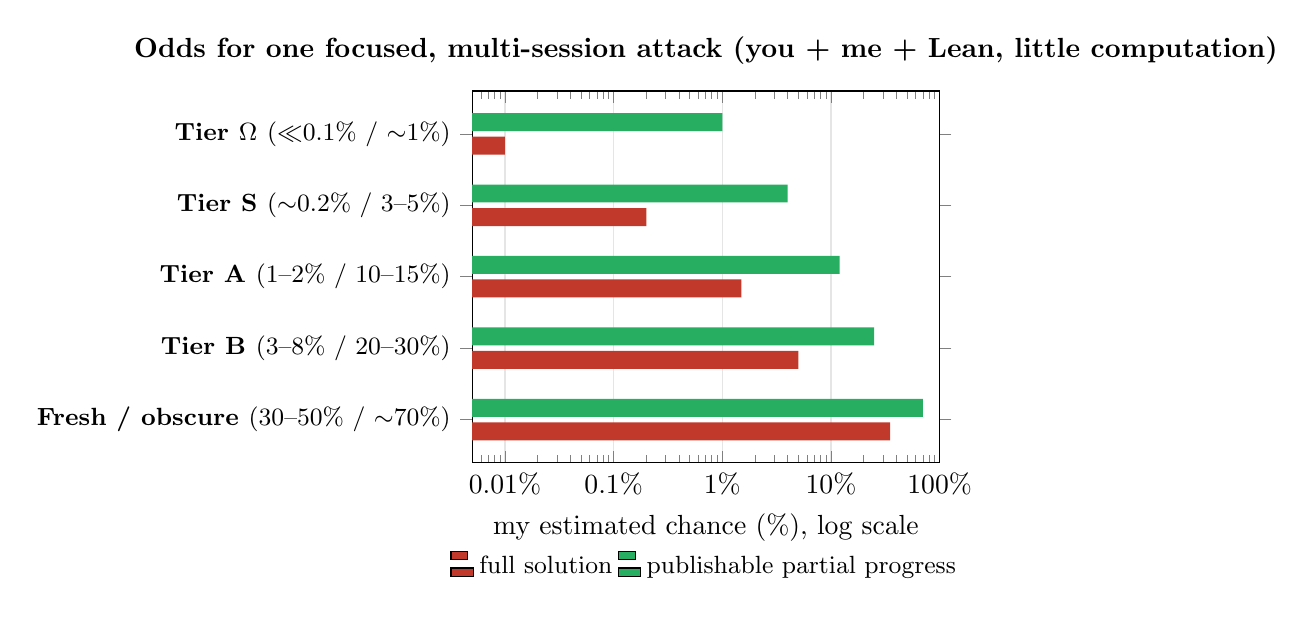
\begin{tikzpicture}
\begin{axis}[xbar, width=0.62\textwidth, height=6.3cm, bar width=6.5pt, xmode=log, log basis x=10,
  xmin=0.005, xmax=100, xlabel={my estimated chance (\%), log scale},
  ytick={0,1,2,3,4}, yticklabels={{Fresh / obscure \textmd{(30--50\% / $\sim$70\%)}},{Tier B \textmd{(3--8\% / 20--30\%)}},{Tier A \textmd{(1--2\% / 10--15\%)}},{Tier S \textmd{($\sim$0.2\% / 3--5\%)}},{Tier $\Omega$ \textmd{($\ll$0.1\% / $\sim$1\%)}}},
  yticklabel style={font=\small\bfseries}, enlarge y limits=0.15,
  xticklabels={,0.01\%,0.1\%,1\%,10\%,100\%}, log origin=infty,
  legend style={at={(0.5,-0.22)},anchor=north,font=\small,draw=none},legend columns=2, legend cell align=left,
  xmajorgrids, grid style={black!10},   title={\bfseries Odds for one focused, multi-session attack (you + me + Lean, little computation)}]
\addplot[fill=tS,draw=none] coordinates {(35,0) (5,1) (1.5,2) (0.2,3) (0.01,4)};
\addplot[fill=tG,draw=none] coordinates {(70,0) (25,1) (12,2) (4,3) (1,4)};
\legend{full solution, publishable partial progress}
\end{axis}
\end{tikzpicture}
\end{center}

\begin{multicols}{2}
\begin{keybox}[title={What being very capable \emph{does} buy us}]{tG}
\small
\begin{itemize}[leftmargin=1em]
\item \textbf{Breadth:} a systematic search for transplants (page~\pageref{sec:transplant}) across every field at once.
\item \textbf{Stamina:} hundreds of small cases, lemmas and reformulations without fatigue.
\item \textbf{Verification:} Lean catches the plausible but wrong proof, which is the classic failure mode on famous problems.
\item \textbf{Track record:} last sessions we resolved OEIS A397683 (apparently first) and proved the binary case of our own Lucas conjecture by hand.
\end{itemize}
\end{keybox}
\columnbreak
\begin{keybox}[title={What it does \emph{not} remove}]{tS}
\small
\begin{itemize}[leftmargin=1em]
\item \textbf{Barriers.} They hold for every solver, however intelligent.
\item \textbf{Missing theories.} Langlands-type problems need decades of new concepts, not one argument.
\item \textbf{Novelty risk.} It is easy to re-prove something known, as happened twice before; a literature check comes first.
\item \textbf{Overconfidence.} Long ``proofs'' of famous conjectures are almost always wrong. Lean is our safeguard, and the reason I will not claim a proof I cannot check.
\end{itemize}
\end{keybox}
\end{multicols}

\noindent\textbf{Revision (9 Oct 2026).} The odds above were written before I had read this year's news, and
for the top tiers they are too pessimistic \emph{about what is possible}. The Navier--Stokes claim shows that
Tier~$\Omega$ is reachable in principle. What the chart still measures is \emph{our} setup: OpenAI's proof used
about 10{,}000 agents for 88 hours (millions of dollars), and our rule is minimal computation. With reasoning
alone, the gap is our compute budget, not a law of nature.

\noindent\textbf{Bottom line.} Attacking a Tier~$\Omega$ problem head-on, \emph{with our budget}, is still a long shot. A Tier~A or B
problem in the sweet spot is a real bet with meaningful odds, and even partial progress there (a better constant,
a new special case, or a clean reformulation) is publishable. If you want a moonshot, choose one that shares
structure with work we have already done: Frege lower bounds connect directly to our naming calculus.

% =====================================================================
\newpage
\section{My picks: where I would attack}\label{sec:picks}

Ordered from the best bet to the boldest. ``Lean ready'' means a formal statement already exists in the local
\texttt{formal-conjectures} library, so we can start proving at once.

\begin{tcbraster}[raster columns=2,raster equal height=rows,raster column skip=8pt,raster row skip=8pt]
\begin{card}{tA}{1. Union-closed sets (Frankl, 1979)}
\textbf{Claim:} in every union-closed family, some element lies in at least half of the sets.\\
\textbf{Why it fits:} Gilmer's 2022 entropy proof of a constant fraction is about 8 pages, and the problem is
pure finite combinatorics. \emph{Lean ready.}\\
\textbf{The wall:} single-coupling entropy arguments provably stall near $0.382$.\\
\textbf{First move:} two-step couplings, or entropy combined with a compression/shifting argument; test only on tiny families.
\end{card}
\begin{card}{tA}{2. \v{C}ern\'y conjecture (1964)}
\textbf{Claim:} a synchronizing $n$-state automaton has a reset word of length $\le(n-1)^2$.\\
\textbf{Why it fits:} a clean statement about words and subsets; the progress has been combinatorial. \emph{Lean ready.}\\
\textbf{The wall:} 60 years stuck at about $n^3/6$.\\
\textbf{First move:} a potential function on subsets that provably shrinks every $n$ steps, in the same spirit as our speed-limit potentials.
\end{card}
\begin{card}{tS}{3. New: audit and understand an AI claim}
\textbf{What:} take one claimed result with a Lean proof, such as Seymour's conjecture (OAI 173) or Erd\H{o}s's
progression conjecture (OAI 159, whose Lean file proves less than the paper claims).\\
\textbf{Do:} check that the Lean statement is the real conjecture, find any gap, and write the short human proof.\\
\textbf{Why:} real value, high odds, and nobody owns this niche yet.
\end{card}
\begin{card}{tB}{4. The 1/3--2/3 conjecture (1968)}
\textbf{Claim:} every finite non-chain poset has a pair $x,y$ with $\tfrac13\le\Pr[x<y]\le\tfrac23$.\\
\textbf{Why it fits:} a geometric inequality on order polytopes; the 0.276 bound came from Brunn--Minkowski. \emph{Lean ready.}\\
\textbf{First move:} transplant a sharper log-concavity tool (Lorentzian polynomials, 2020) to beat 0.276.
\end{card}
\begin{card}{tB}{5. Erd\H{o}s--Gy\'arf\'as (1995)}
\textbf{Claim:} every graph of minimum degree 3 contains a cycle whose length is a power of 2.\\
\textbf{First move:} the structure of a minimal counterexample, plus parity arguments in the cycle space over $\mathbb F_2$.
\end{card}
\begin{card}{tS}{6. Sunflower conjecture (1960)}
\textbf{Claim:} $k$-uniform families with no 3-sunflower have size at most $C^k$.\\
\textbf{Why it fits:} 2019 brought a leap through ``spread'' sets in a short paper; the 3-petal case touches cap sets. \emph{Lean ready.}\\
\textbf{First move:} combine slice-rank (cap sets) with spread sets.
\end{card}
\begin{card}{tS}{7. Moonshot: Frege lower bounds}
\textbf{Why us:} our naming calculus is a model of the copying-versus-naming gap that \emph{is} Frege vs Extended Frege.\\
\textbf{Realistic sub-target:} lower bounds for $\mathrm{AC}^0[p]$-Frege (bounded depth with mod-$p$ gates), open since the 1990s and Tier~A in its own right.
\end{card}
\begin{card}{tC}{8. Warm-up that is ours: the Lucas conjecture}
Finish what we started: formalise the binary case $u<7\varphi^{C/3}$ in Lean, then attack windows of size
$\le3$ by block amortisation. Nobody else is working on it, because we posed it.
\end{card}
\end{tcbraster}

\begin{keybox}[title={Proposed plan for the hard-problem session}]{tO}
\begin{enumerate}[leftmargin=1.3em]
\item \textbf{You choose} one target from cards 1--6 (my vote: \textbf{union-closed sets}, or card~3 for the safest real contribution).
\item \textbf{Literature sweep first}, now including \texttt{openai/math}, \texttt{openai/ten-proofs} and erdosproblems.com, so that we never re-prove a known (or freshly claimed) result.
\item \textbf{Transplant brainstorm:} list 10--15 tools from distant fields with the right shape and kill most of
  them quickly with small, cheap examples.
\item \textbf{Aim for a ladder of results:} a new special case, then a better constant, then the full conjecture.
  Every rung is formalised in Lean before we claim it.
\item \textbf{Write it up honestly}, including the dead ends, which other researchers find valuable too.
\end{enumerate}
\end{keybox}

\end{document}
